\documentclass[11pt,a4paper]{article}

\usepackage[margin=1 in]{geometry}
\usepackage{amsfonts,amsmath,amssymb}
\usepackage[none]{hyphenat}
\usepackage{fancyhdr}
\usepackage{graphicx}
\usepackage{tikz}
\usetikzlibrary{arrows.meta}

% ---------------------------------------------------------------------------
% House diagram style - the same one the probability notes use, so the two
% courses look like they came from the same book. Colours match the accents in
% the web stylesheet; the weight keywords are flattened so no diagram shouts
% next to its neighbour; arrow tips are set once for every picture.
% ---------------------------------------------------------------------------
\definecolor{blue}{HTML}{1D4ED8}
\definecolor{red}{HTML}{B91C1C}
\definecolor{green}{HTML}{12603F}
\definecolor{orange}{HTML}{A16207}
\definecolor{gray}{HTML}{6B7280}

\tikzset{
  every picture/.style={font=\small, line join=round, line cap=round, >=Stealth},
  thin/.style={line width=0.5pt},
  thick/.style={line width=0.9pt},
  very thick/.style={line width=1.1pt},
  ultra thick/.style={line width=1.3pt},
}
\usepackage{color}
\usepackage{xcolor}
\usepackage{array}
\usepackage{float}
\usepackage{multirow}
\usepackage{soul}
\usepackage[nottoc,notlot,notlof]{tocbibind}


% ---------------------------------------------------------------------------
% Tally marks.
%
% These were \StrokeOne .. \StrokeFive from ifsym, which is not installed here
% (it lives in texlive-fonts-extra). Rather than add a dependency that may be
% missing on the next machine, they are drawn with TikZ, which is already
% loaded and which tex4ht converts to SVG for the web.
%
% They matter: the frequency-table sections use them to show how raw
% observations become counts, which is the whole point of the first tally
% column. Dropping them would remove the step being taught.
% ---------------------------------------------------------------------------
\newcommand{\tallystroke}[1]{\draw[line width=.7pt] (#1*0.16,0) -- (#1*0.16,0.32);}
\newcommand{\tallybox}[1]{%
  \raisebox{-0.02em}{\begin{tikzpicture}[baseline=0pt,inner sep=0pt]#1\end{tikzpicture}}%
}
\newcommand{\StrokeOne}  {\tallybox{\tallystroke{0}}}
\newcommand{\StrokeTwo}  {\tallybox{\tallystroke{0}\tallystroke{1}}}
\newcommand{\StrokeThree}{\tallybox{\tallystroke{0}\tallystroke{1}\tallystroke{2}}}
\newcommand{\StrokeFour} {\tallybox{\tallystroke{0}\tallystroke{1}\tallystroke{2}\tallystroke{3}}}
% the fifth stroke crosses the other four, as a tally is actually written
\newcommand{\StrokeFive} {\tallybox{%
  \tallystroke{0}\tallystroke{1}\tallystroke{2}\tallystroke{3}%
  \draw[line width=.7pt] (-0.06,0.04) -- (0.54,0.28);}}



\parindent 0ex

\usetikzlibrary{arrows.meta,shapes,trees,bending,graphs,patterns,quotes,angles}

\pagestyle{fancy}
\fancyhead[R]{}
\renewcommand{\headrulewidth}{0pt}
\fancyfoot[C]{{Page} \thepage}


% ---------------------------------------------------------------------------
% Practice problems, as in the probability notes. These notes define no
% theorem-like environments of their own, so amsthm is loaded here for them.
% build.py collapses each solution into a <details> block on the web, so a
% problem can be attempted before the answer is visible.
% ---------------------------------------------------------------------------
\usepackage{amsthm}
\theoremstyle{definition}
% a plain Definition environment - build.py colours it blue on the web, the
% same as the probability notes
\newtheorem{thm}{Theorem}[section]
\newtheorem{definition}[thm]{Definition}
\newtheorem{example}[thm]{Example}
\newtheorem{exe}[thm]{Exercise}
\newtheorem{note}[thm]{Note}
\newtheorem{remark}[thm]{Remark}
\newtheorem{problemx}{Problem}[section]
\newenvironment{problem}[1]
  {\begin{problemx}\textup{\small[#1]}\hspace{0.4em}\ignorespaces}
  {\end{problemx}}
\newenvironment{solution}
  {\renewcommand{\qedsymbol}{}\begin{proof}[\textit{Solution}.]}
  {\end{proof}}

% Table rows were padded out with empty '&&&\\' rows to fake vertical
% space. Those render as blank rows on the web; set the spacing properly
% once instead.
\renewcommand{\arraystretch}{1.25}

\begin{document}
% Same treatment as the other courses: no name, no university, no lecturer, no
% course code. The material is not specific to one institution.
\begin{titlepage}
\begin{center}
\vspace*{4cm}
{\Huge\bfseries Foundation Mathematics}\\[1.2cm]
{\large Lecture Notes}\\[3cm]
\line(1,0){300}
\end{center}
\end{titlepage}

\tableofcontents
\thispagestyle{empty}
\clearpage
\setcounter{page}{1}


\section{Sets}

Almost everything later in this course is described using sets, so it is worth
being careful here even though the ideas are simple. By the end of this chapter you
should be able to say exactly what a set is, write one in two different notations,
combine sets with the four operations, draw and read a Venn diagram, and use the
laws of set algebra to simplify an expression.

\subsection{What a set is}

\begin{definition}
A \textbf{set} is a collection of well defined objects. The objects in it are
called its \textbf{elements} or \textbf{members}. A set is written by listing its
elements inside braces, $\{\ \}$.
\end{definition}

The phrase \emph{well defined} is doing real work. It means there must be no
argument about whether a given object is in the set. ``The set of whole numbers
between $1$ and $6$'' is well defined; ``the set of interesting numbers'' is not,
because nobody can settle whether $7$ belongs.

\begin{example}
The set containing $1$, $2$, $3$ and $4$ is written $\{1,2,3,4\}$.
\end{example}

Two conventions to fix straight away.

\begin{note}
\textbf{Order does not matter} and \textbf{repetition does not count}. The sets
$\{1,2,3\}$, $\{3,1,2\}$ and $\{1,2,2,3\}$ are all the same set. A set records only
\emph{which} objects are in it.
\end{note}

Sets are named with capital letters and their elements usually with small letters.
To say an object belongs to a set we use the symbol $\in$, and to say it does not we
strike it through:
$$4\in\{1,2,3,4\},\qquad 7\notin\{1,2,3,4\}.$$
Read $\in$ as ``is an element of''.

\subsubsection{Set-builder notation}

Listing works when there are a few elements. For larger sets we describe the
elements instead.

\begin{definition}
\textbf{Set-builder notation} writes a set as
$$\{x : \text{condition on } x\}$$
read ``the set of all $x$ such that \dots''. The colon may be written as a vertical
bar, $\{x \mid \dots\}$; the two mean the same thing.
\end{definition}

\begin{table}[H]
\centering
\begin{tabular}{|l|l|}
\hline
Listed & Described\\
\hline
$A=\{1,2,3,4,5\}$ & $A=\{x : x \text{ is a natural number less than } 6\}$\\
$V=\{a,e,i,o,u\}$ & $V=\{x : x \text{ is a vowel}\}$\\
$C=\{2,4,6,8,10,\ldots\}$ & $C=\{x : x \text{ is a positive even number}\}$\\
\hline
\end{tabular}
\caption{The same sets in both notations. Either description lets you decide what belongs.}
\end{table}

Not every collection can be written both ways. A set such as
$\{\text{dog},\ \text{plate},\ \text{Earth}\}$ has no property in common to describe,
so listing is the only option --- which is fine.

\begin{example}
List the elements of each set.
\begin{enumerate}
\item[(a).] $A=\{x : x \text{ is an odd natural number}\}$
\item[(b).] $B=\{k : k=3n+1,\ n=0,1,2,3\}$
\item[(c).] $D=\{x : x \text{ is a month whose name begins with } J\}$
\end{enumerate}
\end{example}

\begin{solution}
\textbf{(a)} $A=\{1,3,5,7,9,\ldots\}$. The three dots mean the pattern continues
without end; this set is infinite.

\textbf{(b)} Here $n$ is given four values, so substitute each one in turn:
$$n=0:\ 3(0)+1=1,\quad n=1:\ 3(1)+1=4,\quad n=2:\ 3(2)+1=7,\quad n=3:\ 3(3)+1=10.$$
$$\therefore\quad B=\{1,4,7,10\}.$$

\textbf{(c)} $D=\{\text{January},\ \text{June},\ \text{July}\}$.
\end{solution}

\subsubsection{Kinds of set}

\begin{definition}
A set is \textbf{finite} if its elements can be counted and the counting stops. It is
\textbf{infinite} if the counting never stops.
\end{definition}

$V=\{x:x\text{ is a vowel}\}$ is finite; $C=\{2,4,6,\ldots\}$ is infinite.

\begin{definition}
The \textbf{universal set}, written $U$ or $E$, is the set of everything under
discussion in a particular problem.
\end{definition}

The universal set is not fixed once and for all --- it is chosen to suit the
question. In a problem about a class of students, $U$ is that class; in a problem
about digits, $U=\{0,1,2,\ldots,9\}$. It matters because complements depend on it.

\begin{definition}
The \textbf{empty set} or \textbf{null set} contains no elements at all. It is
written $\varnothing$ or $\{\ \}$.
\end{definition}

\begin{remark}
$\{\varnothing\}$ is \textbf{not} the empty set. It is a set with one element, and
that element happens to be the empty set. Compare an empty box with a box containing
an empty box: the second is not empty. So
$$|\varnothing|=0\qquad\text{but}\qquad |\{\varnothing\}|=1.$$
\end{remark}

\subsubsection{Subsets and equality}

\begin{definition}
$S$ is a \textbf{subset} of $T$, written $S\subseteq T$, if every element of $S$ is
also an element of $T$. If in addition $T$ has at least one element that $S$ does not,
then $S$ is a \textbf{proper subset} of $T$, written $S\subset T$.
\end{definition}

\begin{example}
Let $A=\{a,b,c\}$, $B=\{a,b,c,d\}$ and $C=\{2,5,9\}$, $D=\{2,3,5,6,9,10\}$. Then
$A\subset B$ and $C\subset D$, both proper, since $d\in B$ but $d\notin A$, and
$3\in D$ but $3\notin C$.
\end{example}

\begin{note}
Two facts that look strange the first time and are used constantly afterwards:
$$\varnothing\subseteq A\quad\text{for every set } A,\qquad\text{and}\qquad A\subseteq A.$$
The first holds because to fail, $\varnothing$ would need an element that is not in
$A$ --- and it has no elements to offer. The second is immediate from the definition.
\end{note}

\begin{definition}
Sets $A$ and $B$ are \textbf{equal}, written $A=B$, if they have exactly the same
elements. Equivalently, $A=B$ precisely when $A\subseteq B$ and $B\subseteq A$.
\end{definition}

That second form is how equality of sets is usually \emph{proved}: show each is
contained in the other.

\begin{example}
If $A=\{a,b,c\}$ and $B=\{a,c,b\}$ then $A=B$, since order does not matter.
\end{example}

\subsubsection{Cardinality and the power set}

\begin{definition}
The \textbf{cardinality} of a finite set $A$, written $n(A)$ or $|A|$, is the number
of elements it contains. The \textbf{power set} of $A$, written $P(A)$, is the set of
\emph{all} subsets of $A$.
\end{definition}

\begin{example}
Find the power set of each of the following, and its cardinality.
\begin{enumerate}
\item[(a).] $A=\varnothing$
\item[(b).] $B=\{1,2\}$
\item[(c).] $T=\{p,q,r\}$
\end{enumerate}
\end{example}

\begin{solution}
\textbf{(a)} The only subset of the empty set is the empty set itself, so
$$P(A)=\{\varnothing\},\qquad |P(A)|=1.$$
Note again that $P(A)$ here is not empty --- it has one member.

\textbf{(b)} Take the subsets by size: none, one element, two elements.
$$P(B)=\big\{\varnothing,\ \{1\},\ \{2\},\ \{1,2\}\big\},\qquad |P(B)|=4.$$

\textbf{(c)} Same method, now with four sizes:
$$P(T)=\big\{\varnothing,\ \{p\},\ \{q\},\ \{r\},\ \{p,q\},\ \{p,r\},\ \{q,r\},\ \{p,q,r\}\big\},
\qquad |P(T)|=8.$$
\end{solution}

The three answers were $1$, $4$ and $8$ for sets of size $0$, $2$ and $3$. That is
not a coincidence.

\begin{note}
If a set has $n$ elements, its power set has $\boldsymbol{2^n}$ members.

The reason is worth a moment, because it saves listing. Building a subset means
going through the elements one at a time and deciding, for each, whether to put it in
or leave it out. That is $n$ decisions with two answers each, so the number of
different subsets is
$$\underbrace{2\times 2\times\cdots\times 2}_{n\ \text{times}}=2^n.$$
\end{note}

Check it against the example above: $2^0=1$, $2^2=4$ and $2^3=8$. All three agree. It
also tells you when you have finished listing --- a set of $4$ elements must have
$16$ subsets, so if you have written down $15$ you have missed one.

\subsection{Operations on sets}

Throughout this section $U$ is the universal set.

\begin{definition}
Let $A$ and $B$ be sets.
\begin{enumerate}
\item[(i).] The \textbf{complement} of $A$, written $A^c$, is everything in $U$ that
is not in $A$:
$$A^c=\{x : x\in U \text{ and } x\notin A\}.$$
\item[(ii).] The \textbf{union} $A\cup B$ is everything in $A$ or in $B$ or in both:
$$A\cup B=\{x : x\in A \text{ or } x\in B\}.$$
\item[(iii).] The \textbf{intersection} $A\cap B$ is everything in both:
$$A\cap B=\{x : x\in A \text{ and } x\in B\}.$$
\item[(iv).] The \textbf{difference} $A-B$ is everything in $A$ but not in $B$:
$$A-B=\{x : x\in A \text{ and } x\notin B\}.$$
\end{enumerate}
\end{definition}

\begin{note}
The ``or'' in a union is \textbf{inclusive} --- it means \emph{or both}, not
\emph{either but not both}. This is not how ``or'' is always used in ordinary
speech, and it is the commonest source of early mistakes.
\end{note}

Two relationships worth noticing at once:
$$A-B=A\cap B^c,\qquad\text{and}\qquad A\cup A^c=U,\quad A\cap A^c=\varnothing.$$
The first says that taking away $B$ is the same as keeping only what is outside $B$;
it is often the easier of the two to compute with.

\begin{definition}
$A$ and $B$ are \textbf{disjoint} if $A\cap B=\varnothing$, that is, if they have no
element in common.
\end{definition}

\begin{example}
Let $U=\{1,2,3,4,5,6,7,8,9,10\}$, $A=\{2,3,4,5\}$ and $B=\{1,3,4,6\}$. Find
$$\text{(a) } A^c,\qquad \text{(b) } A\cup B,\qquad \text{(c) } A\cap B,
\qquad \text{(d) } A-B,\qquad \text{(e) } (A\cup B)^c.$$
\end{example}

\begin{solution}
\textbf{(a)} Everything in $U$ that is missing from $A$:
$$A^c=\{1,6,7,8,9,10\}.$$

\textbf{(b)} Everything appearing in either set, each listed once:
$$A\cup B=\{1,2,3,4,5,6\}.$$

\textbf{(c)} Only what appears in both:
$$A\cap B=\{3,4\}.$$

\textbf{(d)} Start from $A=\{2,3,4,5\}$ and remove anything also in $B$; that removes
$3$ and $4$:
$$A-B=\{2,5\}.$$
The same answer via $A\cap B^c$: here $B^c=\{2,5,7,8,9,10\}$, and intersecting with
$A$ gives $\{2,5\}$ as before.

\textbf{(e)} From (b), $A\cup B=\{1,2,3,4,5,6\}$, so
$$(A\cup B)^c=\{7,8,9,10\}.$$
\end{solution}

\subsubsection{Venn diagrams}

A \textbf{Venn diagram} draws the universal set as a rectangle and each set inside it
as a circle. Overlaps show elements the sets share. They are the quickest way to see
what a complicated expression means.

\begin{figure}[H]
\centering
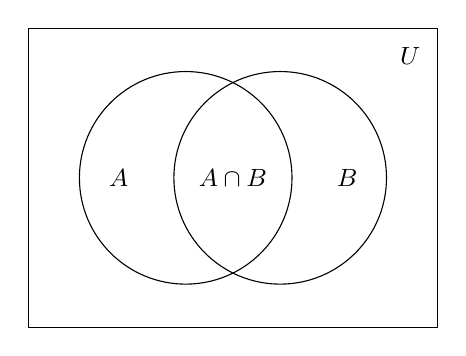
\begin{tikzpicture}
\draw (-2.6,-1.9) rectangle (2.6,1.9);
\node at (2.25,1.55) {$U$};
\draw (-0.6,0) circle (1.35);
\draw (0.6,0) circle (1.35);
\node at (-1.45,0) {$A$};
\node at (1.45,0) {$B$};
\node at (0,0) {$A\cap B$};
\end{tikzpicture}
\caption{Two sets. The whole shaded-looking region inside both circles is $A\cup B$; the overlap alone is $A\cap B$; everything outside both circles but inside the rectangle is $(A\cup B)^c$.}
\end{figure}

With three sets the picture has eight regions --- seven inside the circles and one
outside them all. Every element of $U$ lies in exactly one of them, which is what
makes the diagram useful for counting.

\begin{figure}[H]
\centering
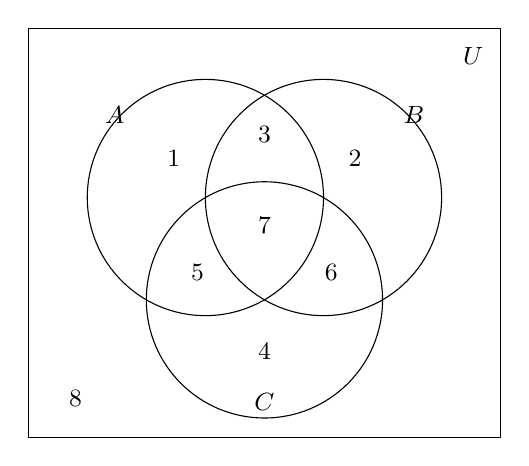
\begin{tikzpicture}
\draw (-3,-2.6) rectangle (3,2.6);
\node at (2.65,2.25) {$U$};
\draw (-0.75,0.45) circle (1.5);
\draw (0.75,0.45) circle (1.5);
\draw (0,-0.85) circle (1.5);
\node at (-1.9,1.5) {$A$};
\node at (1.9,1.5) {$B$};
\node at (0,-2.15) {$C$};
\node at (-1.15,0.95) {\small 1};
\node at (1.15,0.95) {\small 2};
\node at (0,1.25) {\small 3};
\node at (0,-1.5) {\small 4};
\node at (-0.85,-0.5) {\small 5};
\node at (0.85,-0.5) {\small 6};
\node at (0,0.1) {\small 7};
\node at (-2.4,-2.1) {\small 8};
\end{tikzpicture}
\caption{Three sets divide $U$ into eight regions: 7 is in all three, 3, 5 and 6 are in exactly two, 1, 2 and 4 are in exactly one, and 8 is in none.}
\end{figure}

\begin{example}
Let $U=\{a,b,c,d,e,f,g,h\}$, $A=\{a,c,g\}$, $B=\{b,c,f,g\}$ and $C=\{b,d,e,f,g\}$.
Find (a) $B\cup C$, (b) $A^c$, (c) $A^c\cap(B\cup C)$.
\end{example}

\begin{solution}
\textbf{(a)} Collect everything in either set:
$$B\cup C=\{b,c,d,e,f,g\}.$$

\textbf{(b)} Everything in $U$ but not in $A$:
$$A^c=\{b,d,e,f,h\}.$$

\textbf{(c)} Now intersect the two answers. Work through $A^c$ one element at a time
and keep those also in $B\cup C$: $b$ yes, $d$ yes, $e$ yes, $f$ yes, $h$ no.
$$A^c\cap(B\cup C)=\{b,d,e,f\}.$$
Notice the brackets were done first. Without them, $A^c\cap B\cup C$ would be
ambiguous.
\end{solution}

\subsubsection{Counting with a Venn diagram}

This is the application first-year students meet most often, and the one where a
diagram is not optional --- it is the method.

\begin{example}
A survey of $200$ students asked which of Economics, Statistics and Computing they
were taking. The results were:
\begin{table}[H]
\centering
\begin{tabular}{|l|c|}
\hline
Economics & 90\\
Statistics & 80\\
Computing & 70\\
Economics and Statistics & 35\\
Economics and Computing & 30\\
Statistics and Computing & 25\\
All three & 12\\
\hline
\end{tabular}
\end{table}
\begin{enumerate}
\item[(a).] Represent the information on a Venn diagram.
\item[(b).] How many students take none of the three?
\item[(c).] How many take exactly one?
\item[(d).] How many take exactly two?
\end{enumerate}
\end{example}

\begin{solution}
\textbf{The rule that makes this work: fill the diagram from the middle outwards.}
The figures such as ``$35$ take Economics and Statistics'' include the students who
take all three, so they cannot be written straight into the diagram. Start with the
centre, where the count is unambiguous, and subtract as you move out.

\textbf{Step 1 --- the centre.} All three: $12$.

\textbf{Step 2 --- exactly two.} Each pairwise figure includes the $12$ in the middle,
so remove them:
\begin{align*}
\text{Economics and Statistics only} &= 35-12 = 23\\
\text{Economics and Computing only} &= 30-12 = 18\\
\text{Statistics and Computing only} &= 25-12 = 13
\end{align*}

\textbf{Step 3 --- exactly one.} Each subject total includes everyone taking it,
so remove the three regions already filled inside that circle:
\begin{align*}
\text{Economics only} &= 90-23-18-12 = 37\\
\text{Statistics only} &= 80-23-13-12 = 32\\
\text{Computing only} &= 70-18-13-12 = 27
\end{align*}

\begin{figure}[H]
\centering
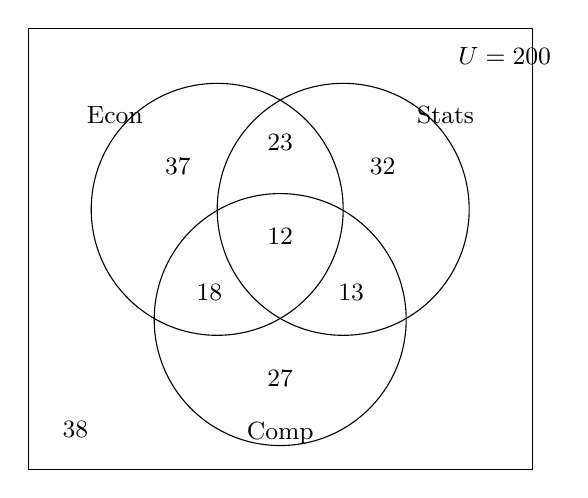
\begin{tikzpicture}
\draw (-3.2,-2.8) rectangle (3.2,2.8);
\node at (2.85,2.45) {$U=200$};
\draw (-0.8,0.5) circle (1.6);
\draw (0.8,0.5) circle (1.6);
\draw (0,-0.9) circle (1.6);
\node at (-2.1,1.7) {Econ};
\node at (2.1,1.7) {Stats};
\node at (0,-2.35) {Comp};
\node at (-1.3,1.05) {37};
\node at (1.3,1.05) {32};
\node at (0,1.35) {23};
\node at (0,-1.65) {27};
\node at (-0.9,-0.55) {18};
\node at (0.9,-0.55) {13};
\node at (0,0.15) {12};
\node at (-2.6,-2.3) {38};
\end{tikzpicture}
\caption{The completed diagram. Every one of the eight regions now holds a count, and they total 200.}
\end{figure}

\textbf{(b)} Add the seven regions inside the circles:
$$37+32+27+23+18+13+12=162,$$
so the number taking none is
$$200-162=38.$$

\textbf{(c)} Exactly one means the three outer regions:
$$37+32+27=96.$$

\textbf{(d)} Exactly two means the three overlap regions, not counting the centre:
$$23+18+13=54.$$

\textbf{Check.} The number taking at least one can also be found without the diagram,
by the \textbf{inclusion--exclusion principle}:
$$n(E\cup S\cup C)=n(E)+n(S)+n(C)-n(E\cap S)-n(E\cap C)-n(S\cap C)+n(E\cap S\cap C)$$
$$=90+80+70-35-30-25+12=162,$$
which agrees. Adding the three totals counts the pairwise overlaps twice, so they are
subtracted; but that removes the centre three times when it was added three times, so
it must be put back once. Getting $162$ by both routes is good evidence the diagram
was filled correctly.
\end{solution}

\begin{remark}
The commonest error in this kind of question is writing $35$ into the
Economics-and-Statistics region directly. Do that and every later figure is wrong,
and the eight regions will not total $200$ --- which is exactly why the total is worth
checking at the end.
\end{remark}

\subsection{Laws of the algebra of sets}

Set operations obey rules much like those of ordinary algebra. For any sets $A$, $B$,
$C$ in a universal set $U$:

\begin{table}[H]
\centering
\begin{tabular}{|l|l|l|}
\hline
Name & For $\cup$ & For $\cap$\\
\hline
Idempotent & $A\cup A=A$ & $A\cap A=A$\\
Commutative & $A\cup B=B\cup A$ & $A\cap B=B\cap A$\\
Associative & $(A\cup B)\cup C=A\cup(B\cup C)$ & $(A\cap B)\cap C=A\cap(B\cap C)$\\
Distributive & $A\cup(B\cap C)=(A\cup B)\cap(A\cup C)$ & $A\cap(B\cup C)=(A\cap B)\cup(A\cap C)$\\
Identity & $A\cup\varnothing=A$ & $A\cap U=A$\\
 & $A\cup U=U$ & $A\cap\varnothing=\varnothing$\\
Complement & $A\cup A^c=U$ & $A\cap A^c=\varnothing$\\
 & $(A^c)^c=A$ & $U^c=\varnothing,\ \varnothing^c=U$\\
De Morgan & $(A\cup B)^c=A^c\cap B^c$ & $(A\cap B)^c=A^c\cup B^c$\\
\hline
\end{tabular}
\caption{The laws of set algebra. Each column mirrors the other with $\cup$ and $\cap$ interchanged, and $\varnothing$ and $U$ interchanged.}
\end{table}

That mirroring is called \textbf{duality}, and it halves the number of laws worth
memorising: learn one column and swap the symbols to get the other.

\begin{note}
\textbf{De Morgan's laws in words.} ``Not (A or B)'' means ``not A and not B''; ``not
(A and B)'' means ``not A or not B''. Notice that the operation \emph{changes} when
the complement is taken through the bracket. Forgetting to change $\cup$ into $\cap$
is the usual slip.
\end{note}

\begin{example}
Verify De Morgan's law $(A\cup B)^c=A^c\cap B^c$ for
$$U=\{1,2,3,4,5,6,7,8\},\quad A=\{1,2,3,4\},\quad B=\{3,4,5,6\}.$$
\end{example}

\begin{solution}
Work out each side separately and compare.

\textbf{Left-hand side.}
$$A\cup B=\{1,2,3,4,5,6\}\quad\implies\quad (A\cup B)^c=\{7,8\}.$$

\textbf{Right-hand side.}
$$A^c=\{5,6,7,8\},\qquad B^c=\{1,2,7,8\}$$
$$\implies\quad A^c\cap B^c=\{7,8\}.$$

Both sides give $\{7,8\}$, so the law holds for these sets.
\end{solution}

\begin{remark}
Checking one example does not \emph{prove} a law --- it only fails to disprove it. A
proof would argue about an arbitrary element $x$: if $x\notin A\cup B$ then $x$ is in
neither $A$ nor $B$, so $x\in A^c$ and $x\in B^c$, hence $x\in A^c\cap B^c$; and the
same reasoning runs backwards. That argument covers every possible set at once, which
no amount of examples can do.
\end{remark}

\begin{example}
Simplify $\left(A^c\cup B\right)^c\cup\left(A\cap B\right)$.
\end{example}

\begin{solution}
Take the outer complement first, using De Morgan:
$$\left(A^c\cup B\right)^c=\left(A^c\right)^c\cap B^c=A\cap B^c.$$
So the expression becomes
$$\left(A\cap B^c\right)\cup\left(A\cap B\right).$$
Both terms contain $A$, so factor it out by the distributive law:
$$=A\cap\left(B^c\cup B\right)=A\cap U=A.$$

The whole expression collapses to $A$. Read on the diagram this is obvious: the first
part is everything in $A$ outside $B$, the second is everything in $A$ inside $B$, and
together they are all of $A$.
\end{solution}

\section{Sets of Numbers}

Numbers arrive in stages, and each stage exists because the one before it could not
do something. Counting needs the natural numbers; recording nothing needs zero;
owing needs the negatives; sharing needs fractions; measuring a diagonal needs
something none of those provide. This chapter names each set and the notation that
goes with it.

\subsection{From counting numbers to real numbers}

\begin{definition}
The \textbf{natural numbers} are the counting numbers,
$$\mathbb{N}=\{1,2,3,4,\ldots\}.$$
Including zero gives the \textbf{whole numbers},
$$W=\{0,1,2,3,4,\ldots\},$$
and including the negatives gives the \textbf{integers},
$$\mathbb{Z}=\{\ldots,-3,-2,-1,0,1,2,3,\ldots\}.$$
\end{definition}

\begin{figure}[H]
\centering
\begin{tikzpicture}
\draw[-Stealth](-4.2,0)--(4.2,0);
\foreach \x in {-3,-2,-1,0,1,2,3}{\draw(\x,-0.12)--(\x,0.12); \node at (\x,-0.45){\small $\x$};}
\end{tikzpicture}
\caption{The integers on a number line. Each is a whole step from the next.}
\end{figure}

Each set contains the one before it:
$$\mathbb{N}\subset W\subset\mathbb{Z}.$$

Dividing one integer by another does not usually give an integer, and that is what the
next set is for.

\begin{definition}
A \textbf{rational number} is any number that can be written as a fraction of two
integers with non-zero denominator:
$$\mathbb{Q}=\left\{\frac{p}{q} : p,q\in\mathbb{Z},\ q\neq 0\right\}.$$
\end{definition}

Every integer is rational, since $-3=\frac{-3}{1}$. So the chain extends:
$$\mathbb{N}\subset W\subset\mathbb{Z}\subset\mathbb{Q}.$$

\begin{remark}
In decimal form a rational number always does one of two things:
\begin{enumerate}
\item[(i).] it \textbf{terminates}, as $\frac{3}{4}=0.75$; or
\item[(ii).] it \textbf{recurs}, as $\frac{23}{11}=2.090909\ldots=2.\overline{09}$,
where the bar marks the block that repeats forever.
\end{enumerate}
Nothing else can happen. A decimal that neither stops nor settles into a repeating
block is not rational.
\end{remark}

That last sentence works in reverse too, and gives a method: any recurring decimal
can be turned back into a fraction.

\begin{example}
Express each recurring decimal as a fraction in its lowest terms.
\begin{enumerate}
\item[(a).] $0.\overline{45}$
\item[(b).] $2.\overline{3}$
\item[(c).] $0.1\overline{6}$
\end{enumerate}
\end{example}

\begin{solution}
The trick in every case is to multiply by a power of $10$ chosen so that the
recurring parts line up, then subtract to cancel them.

\textbf{(a)} The block $45$ has \emph{two} digits, so multiply by $10^2=100$.
\begin{align*}
\text{Let}\quad x &= 0.454545\ldots\\
100x &= 45.454545\ldots
\end{align*}
Subtracting the first line from the second, the endless tails cancel exactly:
$$100x-x=45.454545\ldots-0.454545\ldots=45$$
$$\implies\quad 99x=45\quad\implies\quad x=\frac{45}{99}=\frac{5}{11}.$$

\textbf{(b)} One recurring digit, so multiply by $10$.
\begin{align*}
\text{Let}\quad x &= 2.3333\ldots\\
10x &= 23.3333\ldots
\end{align*}
$$10x-x=21\quad\implies\quad 9x=21\quad\implies\quad x=\frac{21}{9}=\frac{7}{3}.$$

\textbf{(c)} Here the $1$ does not recur but the $6$ does, so \emph{two} multiplications
are needed --- one to step past the non-recurring digit, one to span the block.
\begin{align*}
\text{Let}\quad x &= 0.16666\ldots\\
10x &= 1.6666\ldots\\
100x &= 16.6666\ldots
\end{align*}
Now subtract the second from the third, since those two have matching tails:
$$100x-10x=15\quad\implies\quad 90x=15\quad\implies\quad x=\frac{15}{90}=\frac{1}{6}.$$

\textbf{Check.} $1\div 6=0.1666\ldots$, as required.
\end{solution}

\begin{note}
Subtract the two lines whose \emph{tails match}. In part (c), subtracting $x$ from
$100x$ would not work, because $0.1666\ldots$ and $16.6666\ldots$ do not have the same
digits after the point.
\end{note}

\begin{definition}
The \textbf{real numbers} $\mathbb{R}$ are all the numbers that correspond to points on
a number line. A real number that cannot be written as a fraction of integers is
called \textbf{irrational}.
\end{definition}

Examples of irrational numbers are $\sqrt{2}=1.41421\ldots$, $\sqrt{5}$ and
$\pi=3.14159\ldots$ Their decimals run forever without ever settling into a repeating
block. Together,
$$\mathbb{N}\subset W\subset\mathbb{Z}\subset\mathbb{Q}\subset\mathbb{R},$$
and the irrationals are exactly what is left of $\mathbb{R}$ after $\mathbb{Q}$ is
removed.

\subsection{Interval notation}

A set of real numbers between two endpoints is written as an \textbf{interval}. The
only thing to keep track of is whether the endpoints themselves are included.

\begin{table}[H]
\centering
\begin{tabular}{|l|l|l|}
\hline
Interval & Meaning & In set-builder notation\\
\hline
$[a,b]$ & closed: both ends included & $\{x\in\mathbb{R} : a\leq x\leq b\}$\\
$(a,b)$ & open: neither end included & $\{x\in\mathbb{R} : a< x< b\}$\\
$[a,b)$ & half-open & $\{x\in\mathbb{R} : a\leq x< b\}$\\
$(a,b]$ & half-open & $\{x\in\mathbb{R} : a< x\leq b\}$\\
$[a,\infty)$ & unbounded above & $\{x\in\mathbb{R} : x\geq a\}$\\
$(-\infty,b)$ & unbounded below & $\{x\in\mathbb{R} : x< b\}$\\
\hline
\end{tabular}
\caption{Interval notation. A square bracket includes the endpoint, a round one excludes it.}
\end{table}

\begin{note}
$\infty$ is not a number and can never be included, so it always takes a round
bracket: $[2,\infty)$, never $[2,\infty]$.
\end{note}

\begin{example}
Write each of the following in interval notation.
\begin{enumerate}
\item[(a).] All real numbers from $-1$ up to and including $4$.
\item[(b).] $\{x\in\mathbb{R} : x>7\}$
\item[(c).] All real numbers at most $0$ or at least $3$.
\end{enumerate}
\end{example}

\begin{solution}
\textbf{(a)} $-1$ is excluded by ``from'', $4$ is included by ``and including'':
$[-1,4]$ if $-1$ is meant to be included, and here ``from $-1$'' does include it, so
$$[-1,4].$$

\textbf{(b)} Strictly greater, so the endpoint is out and there is no upper limit:
$$(7,\infty).$$

\textbf{(c)} This is two separate pieces, joined by ``or'' --- a union:
$$(-\infty,0]\cup[3,\infty).$$
\end{solution}

\subsection{Radicals and rational powers}

\begin{definition}
If $a\geq 0$, the \textbf{square root} $\sqrt{a}$ is the non-negative number whose
square is $a$. More generally $a^{1/n}=\sqrt[n]{a}$ and
$a^{m/n}=\sqrt[n]{a^m}=\left(\sqrt[n]{a}\right)^m$.
\end{definition}

The rules that make radicals manageable are
$$\sqrt{ab}=\sqrt{a}\,\sqrt{b},\qquad \sqrt{\frac{a}{b}}=\frac{\sqrt{a}}{\sqrt{b}}
\quad (b\neq 0).$$

\begin{note}
There is no such rule for sums. $\sqrt{a+b}$ is \textbf{not} $\sqrt{a}+\sqrt{b}$. Test
it once and remember it: $\sqrt{9+16}=\sqrt{25}=5$, while $\sqrt{9}+\sqrt{16}=3+4=7$.
\end{note}

\subsubsection{Rationalising the denominator}

A fraction with a radical underneath is awkward to work with and, by convention, is
not left in that form. \textbf{Rationalising} means rewriting it so the denominator is
rational.

\begin{example}
Rationalise the denominator of each.
\begin{enumerate}
\item[(a).] $\dfrac{3}{\sqrt{5}}$
\item[(b).] $\dfrac{2}{\sqrt{7}-\sqrt{3}}$
\item[(c).] $\dfrac{1+\sqrt{2}}{3-\sqrt{2}}$
\end{enumerate}
\end{example}

\begin{solution}
\textbf{(a)} A single radical: multiply top and bottom by it.
$$\frac{3}{\sqrt{5}}=\frac{3}{\sqrt{5}}\times\frac{\sqrt{5}}{\sqrt{5}}
=\frac{3\sqrt{5}}{5}.$$
Multiplying by $\frac{\sqrt5}{\sqrt5}$ is multiplying by $1$, so the value has not
changed --- only its appearance.

\textbf{(b)} Two terms underneath. Multiply by the \textbf{conjugate}, the same
expression with the sign between the terms reversed, because
$(x-y)(x+y)=x^2-y^2$ removes both radicals at once.
$$\frac{2}{\sqrt{7}-\sqrt{3}}\times\frac{\sqrt{7}+\sqrt{3}}{\sqrt{7}+\sqrt{3}}
=\frac{2\left(\sqrt{7}+\sqrt{3}\right)}{\left(\sqrt{7}\right)^2-\left(\sqrt{3}\right)^2}
=\frac{2\left(\sqrt{7}+\sqrt{3}\right)}{7-3}
=\frac{2\left(\sqrt{7}+\sqrt{3}\right)}{4}
=\frac{\sqrt{7}+\sqrt{3}}{2}.$$

\textbf{(c)} Same method; the conjugate of $3-\sqrt{2}$ is $3+\sqrt{2}$.
$$\frac{1+\sqrt{2}}{3-\sqrt{2}}\times\frac{3+\sqrt{2}}{3+\sqrt{2}}
=\frac{\left(1+\sqrt{2}\right)\left(3+\sqrt{2}\right)}{9-2}.$$
Expanding the top:
$$\left(1+\sqrt{2}\right)\left(3+\sqrt{2}\right)
=3+\sqrt{2}+3\sqrt{2}+\left(\sqrt{2}\right)^2
=3+4\sqrt{2}+2=5+4\sqrt{2}.$$
$$\therefore\quad \frac{1+\sqrt{2}}{3-\sqrt{2}}=\frac{5+4\sqrt{2}}{7}.$$

\textbf{Check.} $\frac{1+\sqrt2}{3-\sqrt2}\approx 1.5224$ and
$\frac{5+4\sqrt2}{7}\approx 1.5224$. A quick numerical check like this catches sign
errors in the expansion, and takes seconds.
\end{solution}

\subsection{Complex numbers}

No real number squares to give a negative, so $x^2=-1$ has no real solution. Rather
than stop there, we give that missing number a name.

\begin{definition}
The \textbf{imaginary unit} $i$ is defined by
$$i^2=-1,\qquad\text{that is}\qquad i=\sqrt{-1}.$$
A \textbf{complex number} has the form $z=a+bi$ with $a,b\in\mathbb{R}$. Here $a$ is
the \textbf{real part} and $b$ the \textbf{imaginary part}, written
$\operatorname{Re}(z)=a$ and $\operatorname{Im}(z)=b$.
\end{definition}

\begin{note}
The imaginary part is the real number $b$, not $bi$. For $z=3+4i$,
$\operatorname{Im}(z)=4$.
\end{note}

Two complex numbers are \textbf{equal} exactly when their real parts match and their
imaginary parts match. That single fact turns one complex equation into two real ones,
which is how such equations are usually solved.

\subsubsection{Arithmetic with complex numbers}

Addition and subtraction are done part by part. Multiplication is ordinary expansion,
followed by replacing $i^2$ with $-1$.

\begin{example}
Let $z_1=3+4i$ and $z_2=1-2i$. Find (a) $z_1+z_2$, (b) $z_1-z_2$, (c) $z_1z_2$.
\end{example}

\begin{solution}
\textbf{(a)} Add real to real, imaginary to imaginary:
$$z_1+z_2=(3+1)+(4-2)i=4+2i.$$

\textbf{(b)} $$z_1-z_2=(3-1)+(4-(-2))i=2+6i.$$

\textbf{(c)} Expand as usual:
\begin{align*}
z_1z_2 &=(3+4i)(1-2i)\\
       &=3-6i+4i-8i^2\\
       &=3-2i-8i^2.
\end{align*}
Now use $i^2=-1$, so $-8i^2=-8(-1)=+8$:
$$z_1z_2=3+8-2i=11-2i.$$
\end{solution}

\begin{definition}
The \textbf{conjugate} of $z=a+bi$ is $\bar{z}=a-bi$: the same number with the sign of
the imaginary part reversed.
\end{definition}

The conjugate matters because a number times its conjugate is always real:
$$(a+bi)(a-bi)=a^2-(bi)^2=a^2-b^2i^2=a^2+b^2.$$
That is exactly the tool needed for division --- the same idea as rationalising a
denominator.

\begin{example}
Express $\dfrac{3+4i}{1-2i}$ in the form $a+bi$.
\end{example}

\begin{solution}
Multiply top and bottom by the conjugate of the denominator, $1+2i$:
$$\frac{3+4i}{1-2i}\times\frac{1+2i}{1+2i}=\frac{(3+4i)(1+2i)}{1^2+2^2}.$$

The denominator is now real: $1^2+2^2=5$. Expanding the numerator,
$$(3+4i)(1+2i)=3+6i+4i+8i^2=3+10i-8=-5+10i.$$
$$\therefore\quad \frac{3+4i}{1-2i}=\frac{-5+10i}{5}=-1+2i.$$

\textbf{Check.} Multiply back: $(-1+2i)(1-2i)=-1+2i+2i-4i^2=-1+4i+4=3+4i$, which is
the original numerator. Any division can be checked this way.
\end{solution}

\section{Functions}

A function is a rule that turns one number into another. Almost every later chapter
studies some particular family of them, so it is worth being exact about what the word
means and what can go wrong.

\subsection{Ordered pairs and relations}

\begin{definition}
The \textbf{Cartesian product} of sets $X$ and $Y$, written $X\times Y$ and read
``$X$ cross $Y$'', is the set of all ordered pairs with first entry from $X$ and
second from $Y$:
$$X\times Y=\{(x,y) : x\in X,\ y\in Y\}.$$
\end{definition}

The pairs are \emph{ordered}: $(1,a)$ and $(a,1)$ are different, and in $X\times X$ the
pairs $(1,2)$ and $(2,1)$ are different too.

\begin{example}
Let $A=\{1,2\}$ and $B=\{a,b,c\}$. Write down $A\times B$ and $A\times A$.
\end{example}

\begin{solution}
Take each element of the first set with each element of the second, in turn:
$$A\times B=\{(1,a),\,(1,b),\,(1,c),\,(2,a),\,(2,b),\,(2,c)\}.$$
For $A\times A$ the same rule applies, with $A$ playing both parts:
$$A\times A=\{(1,1),\,(1,2),\,(2,1),\,(2,2)\}.$$

\textbf{Count them as a check.} If $|X|=m$ and $|Y|=n$ then $|X\times Y|=mn$, because
each of the $m$ first entries can be paired with each of the $n$ second entries. Here
$|A\times B|=2\times 3=6$ and $|A\times A|=2\times 2=4$, which matches what was
listed.

That check earns its place: $(1,2)$ and $(2,1)$ are both in $A\times A$ and it is easy
to write one and forget the other, leaving three pairs where there should be four.
\end{solution}

\begin{definition}
A \textbf{relation} $R$ from $X$ to $Y$ is any subset of $X\times Y$. If
$(x,y)\in R$ we say $x$ is related to $y$ and write $x\,R\,y$.
\end{definition}

So a relation is just a rule that links some elements of one set to some elements of
another. $X$ is the \textbf{input set} and $Y$ the \textbf{output set}.

\subsubsection{Classifying relations}

Relations are described by how many arrows leave and arrive at each element.

\begin{table}[H]
\centering
\begin{tabular}{|l|l|}
\hline
Type & Description\\
\hline
One-to-one & each input goes to one output, and no output is used twice\\
Many-to-one & several inputs share the same output\\
One-to-many & one input goes to several outputs\\
Many-to-many & both of the last two happen\\
\hline
\end{tabular}
\caption{The four kinds of relation.}
\end{table}

\begin{example}
Let $X=\{3,5,7\}$ and $Y=\{6,10,14\}$ with the relation ``is a factor of''. Show it on
an arrow diagram and classify it.
\end{example}

\begin{solution}
$3$ divides $6$; $5$ divides $10$; $7$ divides $14$. No other pairs work, since $3$
does not divide $10$ or $14$, and so on.
\begin{figure}[H]
\centering
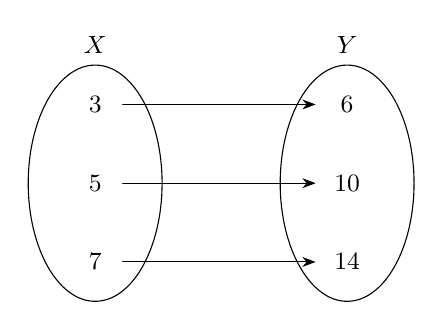
\begin{tikzpicture}
\draw (-1.6,-1.6) ellipse (0.85 and 1.5);
\draw (1.6,-1.6) ellipse (0.85 and 1.5);
\node at (-1.6,0.15) {$X$};
\node at (1.6,0.15) {$Y$};
\foreach \y/\a in {-0.6/3,-1.6/5,-2.6/7}{\node at (-1.6,\y) {$\a$};}
\foreach \y/\b in {-0.6/6,-1.6/10,-2.6/14}{\node at (1.6,\y) {$\b$};}
\foreach \y in {-0.6,-1.6,-2.6}{\draw[-Stealth](-1.25,\y)--(1.2,\y);}
\end{tikzpicture}
\caption{``Is a factor of'' from $X$ to $Y$. One arrow leaves each input and one arrives at each output, so the relation is one-to-one.}
\end{figure}
Every input has exactly one arrow out and every output exactly one arrow in, so the
relation is \textbf{one-to-one}.
\end{solution}

\begin{definition}
For a relation from $X$ to $Y$:
\begin{enumerate}
\item[(i).] the \textbf{domain} is the set of inputs actually used --- the first
entries of the pairs;
\item[(ii).] the \textbf{range} is the set of outputs actually reached --- the second
entries;
\item[(iii).] the \textbf{co-domain} is the whole of $Y$, whether or not every element
of it is reached.
\end{enumerate}
\end{definition}

\begin{note}
The range is always a subset of the co-domain, and often a proper one. The co-domain is
the set you \emph{declared} the outputs would come from; the range is what actually
came out.
\end{note}

\subsection{Functions}

\begin{definition}
A \textbf{function} $f$ from $X$ to $Y$, written $f:X\to Y$, is a relation in which
\emph{every} element of $X$ is assigned to \emph{exactly one} element of $Y$.
\end{definition}

Two conditions, and both matter:

\begin{enumerate}
\item[(i).] \textbf{every} input must be used --- nothing in $X$ is left without an
arrow;
\item[(ii).] each input has \textbf{exactly one} output --- no input has two arrows
leaving it.
\end{enumerate}

So every function is a relation, but not every relation is a function. A one-to-many
relation is never a function, because condition (ii) fails.

We write $y=f(x)$, calling $x$ the \textbf{independent variable} and $y$ the
\textbf{dependent variable}. The value $f(x)$ is read ``$f$ of $x$''.

\begin{note}
$f(x)$ does not mean $f$ multiplied by $x$. It is one symbol meaning ``the output of
$f$ when the input is $x$''.
\end{note}

\begin{example}
The function $f(x)=\frac{x}{2}+7$ is the rule ``halve the input, then add $7$''.
Find $f(4)$, $f(0)$ and $f(-6)$.
\end{example}

\begin{solution}
Substitute each value in turn, keeping the brackets until the last step:
$$f(4)=\frac{4}{2}+7=2+7=9$$
$$f(0)=\frac{0}{2}+7=0+7=7$$
$$f(-6)=\frac{-6}{2}+7=-3+7=4.$$
\end{solution}

\begin{example}
The function $f$ is defined by
$$f(x)=\begin{cases} 2x-3 & \text{for } x<0,\\ 3x+1 & \text{for } x\geq 0.\end{cases}$$
Find $f\!\left(\tfrac{1}{2}\right)$, $f(0)$ and $f(-3)$.
\end{example}

\begin{solution}
This is a \textbf{piecewise} function: which formula applies depends on the input, so
check the condition \emph{first} and only then substitute.

$\tfrac{1}{2}\geq 0$, so use the second line:
$$f\!\left(\tfrac{1}{2}\right)=3\!\left(\tfrac{1}{2}\right)+1=\tfrac{3}{2}+1=\tfrac{5}{2}.$$

$0\geq 0$, so the second line again --- note the condition is $x\geq 0$, not $x>0$:
$$f(0)=3(0)+1=1.$$

$-3<0$, so the first line:
$$f(-3)=2(-3)-3=-6-3=-9.$$

The commonest mistake here is substituting into whichever formula is written first.
Read the condition before choosing the rule.
\end{solution}

\subsection{Composite functions}

\begin{definition}
Given functions $f$ and $g$, the \textbf{composite} $f\circ g$ is defined by
$$(f\circ g)(x)=f\big(g(x)\big).$$
Here $g$ is the \textbf{inside} function and $f$ the \textbf{outside} one.
\end{definition}

Read it from the inside out: apply $g$ first, then feed the answer into $f$. The
notation is the reverse of the order of work, which is what makes it easy to get
backwards.

\begin{example}
Let $f(x)=2x-1$ and $g(x)=3x$. Find
$$\text{(a) } (g\circ f)(x),\qquad \text{(b) } (f\circ g)(x),
\qquad \text{(c) } (f\circ f)(x),\qquad \text{(d) } (g\circ g)(x).$$
\end{example}

\begin{solution}
\textbf{(a)} Inside first: $f(x)=2x-1$. Feed that into $g$, which triples its input:
$$(g\circ f)(x)=g(2x-1)=3(2x-1)=6x-3.$$

\textbf{(b)} Now the other order. Inside is $g(x)=3x$; feed it into $f$, which doubles
and subtracts $1$:
$$(f\circ g)(x)=f(3x)=2(3x)-1=6x-1.$$

\textbf{(c)} $$(f\circ f)(x)=f(2x-1)=2(2x-1)-1=4x-2-1=4x-3.$$

\textbf{(d)} $$(g\circ g)(x)=g(3x)=3(3x)=9x.$$
\end{solution}

\begin{note}
Compare (a) and (b): $6x-3$ against $6x-1$. \textbf{Composition is not commutative} ---
$f\circ g$ and $g\circ f$ are usually different functions. Order matters, and it is not
optional.
\end{note}

\subsection{Odd and even functions}

\begin{definition}
A function $f$ is \textbf{even} if $f(-x)=f(x)$ for every $x$, and \textbf{odd} if
$f(-x)=-f(x)$ for every $x$.
\end{definition}

An even function is unchanged when the sign of the input flips; an odd one changes
sign with it. Graphically, an even function is symmetric about the $y$-axis and an odd
one has rotational symmetry about the origin.

\begin{example}
State whether each function is even, odd, or neither.
\begin{enumerate}
\item[(a).] $f(x)=\dfrac{x^3-x}{x^2+4}$
\item[(b).] $f(x)=x^4-3x^2+7$
\item[(c).] $f(x)=2x+7$
\end{enumerate}
\end{example}

\begin{solution}
In every case the method is the same: work out $f(-x)$, then compare it with $f(x)$ and
with $-f(x)$.

\textbf{(a)} Replace each $x$ by $-x$, remembering $(-x)^3=-x^3$ and $(-x)^2=x^2$:
$$f(-x)=\frac{(-x)^3-(-x)}{(-x)^2+4}=\frac{-x^3+x}{x^2+4}=-\left(\frac{x^3-x}{x^2+4}\right)=-f(x).$$
So $f$ is \textbf{odd}.

\textbf{(b)} Only even powers appear, and the constant is unaffected:
$$f(-x)=(-x)^4-3(-x)^2+7=x^4-3x^2+7=f(x).$$
So $f$ is \textbf{even}.

\textbf{(c)} $$f(-x)=2(-x)+7=-2x+7.$$
This is not $f(x)=2x+7$, so $f$ is not even. Nor is it $-f(x)=-2x-7$, since the
constants differ. So $f$ is \textbf{neither}.
\end{solution}

\begin{note}
Most functions are neither odd nor even --- those two are special cases, not
alternatives. Part (c) shows how a single constant term can spoil oddness: $2x$ on its
own is odd, but $2x+7$ is not.
\end{note}

\subsection{Inverse of a function}

\begin{definition}
Functions $f$ and $g$ are \textbf{inverses} of each other if
$$(f\circ g)(x)=x\quad\text{and}\quad (g\circ f)(x)=x$$
for all $x$ in the appropriate domains. The inverse of $f$ is written $f^{-1}$.
\end{definition}

The inverse undoes what the function does: put a number in, apply $f$, apply $f^{-1}$,
and you are back where you started.

\begin{note}
$f^{-1}$ does \textbf{not} mean $\frac{1}{f}$. The superscript $-1$ here means
``inverse function'', not ``reciprocal''.
\end{note}

Only a one-to-one function has an inverse. If two different inputs shared an output,
the reverse rule would not know which to return, and so would not be a function.

\begin{remark}
Since the inverse reverses every arrow, the domain and range swap over:
$$\text{domain of } f^{-1}=\text{range of } f,\qquad
\text{range of } f^{-1}=\text{domain of } f.$$
\end{remark}

\begin{example}
Show that $f(x)=\dfrac{x-3}{2}$ and $g(x)=2x+3$ are inverses of each other.
\end{example}

\begin{solution}
Both composites must come out as $x$; checking only one is not enough in general.
$$(f\circ g)(x)=f(2x+3)=\frac{(2x+3)-3}{2}=\frac{2x}{2}=x$$
$$(g\circ f)(x)=g\!\left(\frac{x-3}{2}\right)=2\!\left(\frac{x-3}{2}\right)+3=(x-3)+3=x.$$
Both give $x$, so $f$ and $g$ are inverses.
\end{solution}

\subsubsection{Finding an inverse}

The method is always the same three steps: write $y=f(x)$, make $x$ the subject, then
swap the letters.

\begin{example}
Find the inverse of $f(x)=\dfrac{3x+1}{x-2}$, and state its domain.
\end{example}

\begin{solution}
\textbf{Step 1.} Write $y$ for the output:
$$y=\frac{3x+1}{x-2}.$$

\textbf{Step 2.} Make $x$ the subject. Clear the fraction first:
$$y(x-2)=3x+1\quad\implies\quad xy-2y=3x+1.$$
Gather every term containing $x$ on one side and everything else on the other:
$$xy-3x=2y+1\quad\implies\quad x(y-3)=2y+1$$
$$\implies\quad x=\frac{2y+1}{y-3}.$$

\textbf{Step 3.} Swap $x$ and $y$, since the inverse takes the old outputs as its
inputs:
$$f^{-1}(x)=\frac{2x+1}{x-3}.$$

\textbf{Domain.} The inverse is undefined where its denominator vanishes, so
$x\neq 3$; its domain is $\mathbb{R}\setminus\{3\}$. Notice that $3$ is precisely the
value $f$ can never output --- as $x$ grows, $\frac{3x+1}{x-2}$ approaches $3$ without
reaching it. The range of $f$ and the domain of $f^{-1}$ agree, as they must.

\textbf{Check.} $$f\big(f^{-1}(x)\big)
=\frac{3\left(\frac{2x+1}{x-3}\right)+1}{\left(\frac{2x+1}{x-3}\right)-2}
=\frac{\frac{6x+3+x-3}{x-3}}{\frac{2x+1-2x+6}{x-3}}
=\frac{7x}{7}=x. $$
\end{solution}

\end{document}
